$if(has-frontmatter)$
\frontmatter
$endif$
% Page de couverture : image de la densité corrigée en arrière-plan, titre dans la zone blanche du golfe
\begin{titlepage}
\begin{tikzpicture}[remember picture, overlay]
  \node[anchor=south east, inner sep=0pt] at ([xshift=1.2cm, yshift=1.4cm]current page.south east)
    {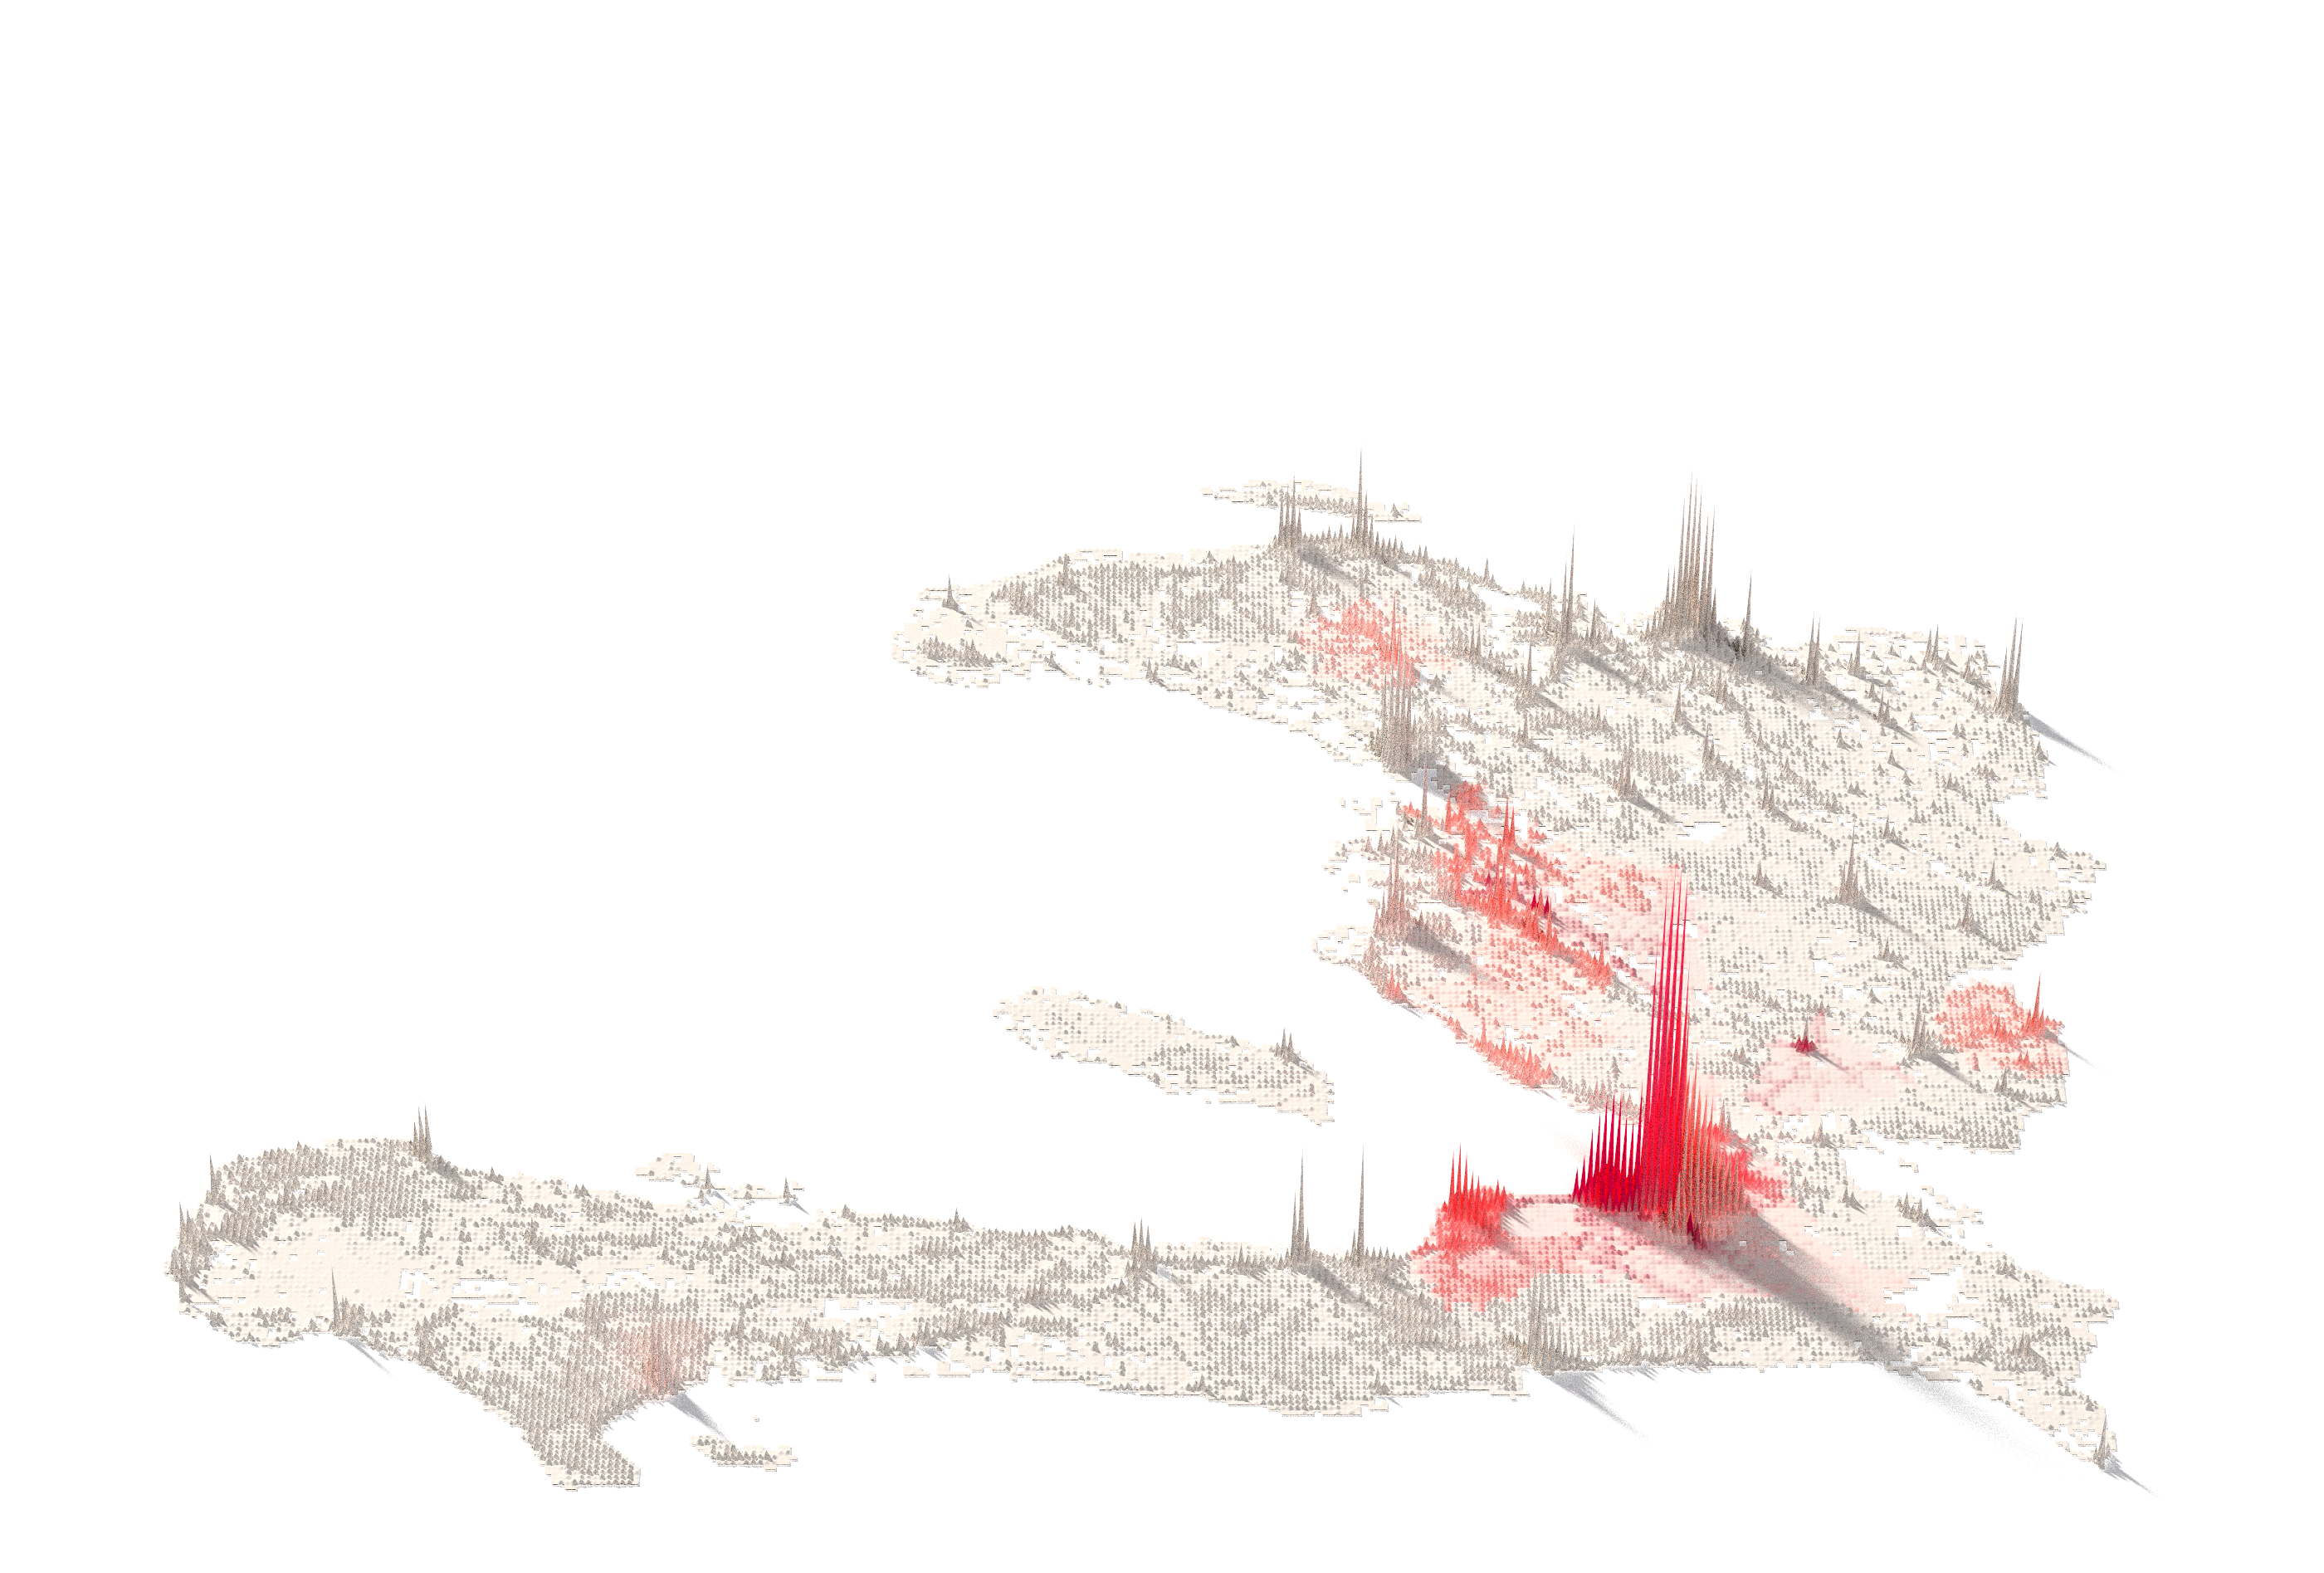
\includegraphics[width=1.15\paperwidth]{figures/rendus/haiti_violence_finale.png}};
  \fill[couvrouge] ([xshift=2.5cm, yshift=-3.4cm]current page.north west) rectangle ++(1.8cm, -0.14cm);
  \node[anchor=north west, inner sep=0pt, text width=15.5cm, align=left]
    at ([xshift=2.5cm, yshift=-4.1cm]current page.north west) {%
    \hyphenpenalty=10000\exhyphenpenalty=10000
    {\sffamily\bfseries\fontsize{28}{34}\selectfont\color{couvencre} $title$\par}
$if(subtitle)$
    \vspace{0.55cm}
    {\fontsize{13}{17}\selectfont\color{couvgris} $subtitle$\par}
$endif$
    \vspace{1.1cm}
    {\sffamily\fontsize{12}{17}\selectfont\color{couvencre} $for(authors)$$it.name.literal$$sep$\par $endfor$\par}
    \vspace{0.3cm}
    {\sffamily\fontsize{10}{13}\selectfont\color{couvgris} $date$\par}
  };
  \node[anchor=south west, inner sep=0pt, text width=15.5cm, align=left, font=\sffamily\scriptsize\color{couvgris}]
    at ([xshift=2.5cm, yshift=0.9cm]current page.south west)
    {Image : densité de population corrigée des déplacements, juillet 2026 (hauteur des pics, cellules de 1 km²) ; en rouge, écart de densité associé à la violence des gangs selon le modèle. Calculs des auteurs.};
\end{tikzpicture}
\end{titlepage}
\pagenumbering{roman}
$if(abstract)$
\begin{abstract}
$abstract$
\end{abstract}
$endif$
